%%%%%%%%%%%%%%%%%%%%%%%%%%%%%%%%%%%%%%%%%%%%%%%%%%%%%%%%%%%%%%%%%%%%%%
% Overleaf (WriteLaTeX) Example: Molecular Chemistry Presentation
%
% Source: http://www.overleaf.com
%
% In these slides we show how Overleaf can be used with standard
% chemistry packages to easily create professional presentations.
%
% Feel free to distribute this example, but please keep the referral
% to overleaf.com
%
%%%%%%%%%%%%%%%%%%%%%%%%%%%%%%%%%%%%%%%%%%%%%%%%%%%%%%%%%%%%%%%%%%%%%%
% How to use Overleaf:
%
% You edit the source code here on the left, and the preview on the
% right shows you the result within a few seconds.
%
% Bookmark this page and share the URL with your co-authors. They can
% edit at the same time!
%
% You can upload figures, bibliographies, custom classes and
% styles using the files menu.
%
% If you're new to LaTeX, the wikibook is a great place to start:
% http://en.wikibooks.org/wiki/LaTeX
%
%%%%%%%%%%%%%%%%%%%%%%%%%%%%%%%%%%%%%%%%%%%%%%%%%%%%%%%%%%%%%%%%%%%%%%

\documentclass[xcolor=table]{beamer}

% For more themes, color themes and font themes, see:
% http://deic.uab.es/~iblanes/beamer_gallery/index_by_theme.html
%
\mode<presentation>
{
  \usetheme{Madrid}       % or try default, Darmstadt, Warsaw, ...
  \usecolortheme{default} % or try albatross, beaver, crane, ...
  \usefonttheme{serif}    % or try default, structurebold, ...
  \setbeamertemplate{navigation symbols}{}
  \setbeamertemplate{caption}[numbered]
}
% \usepackage[table]{xcolor}

% \usepackage[english]{babel}
\usepackage[utf8x]{inputenc}
% \usepackage{chemfig}
% \usepackage{listings}



% On Overleaf, these lines give you sharper preview images.
% You might want to `comment them out before you export, though.
\usepackage{pgfpages}
\pgfpagesuselayout{resize to}[%
  physical paper width=8in, physical paper height=6in]

% Here's where the presentation starts, with the info for the title slide
\title[GPSMO]{General Purpose Molecular Simulation Objects}
\subtitle[]{System Requirements Specification}
\author[Quach et. al.]{Co Quach \\ Justin Gilmer \\  Parashara Shamaprasad \\ Ray Matsumoto \\ Umesh Timalsina}
\institute[MoSDeF]{MoSDeF}
\date{\today}

\begin{document}

\begin{frame}
  \titlepage
\end{frame}

% These three lines create an automatically generated table of contents.
\begin{frame}{Outline}
  \tableofcontents
\end{frame}

\section{Overview}
\begin{frame}{Overview}
\begin{itemize}
\item Define the goals, objectives, constructs and major capabilities expected of \textbf{GPMSO} specification

\item Specify
    \begin{itemize}
        \item Functional requirements
        \item Data requirements
        \item Constraints
    \end{itemize}
\item Intended use
    \begin{itemize}
        \item For software developers/research engineers/research scientists looking to represent a molecular system (parameterized or non-parameterized)
        \item Simulationists using molecular simulation engines
    \end{itemize}

\end{itemize}
\end{frame}

\section{Introduction}
\begin{frame}{Introduction}
    \begin{itemize}
        \item Provide a general specification of a GPMSO molecular system and the constructs necessary to accomplish this
        \begin{itemize}
            \item Living document, can be updated over time
        \end{itemize}
        \item Base data structures that are general enough to support as many chemical systems and interaction forms as needed

        \item Two \textbf{container} objects required
        \begin{itemize}
            \item \texttt{System} -- Physical representations stored here \\
            - \texttt{Site}, \texttt{Connection}, etc...
            \item \texttt{PotentialCollection} --  non-physical representations stored here \\
            - Functional form of interaction, parameters, etc...

        \end{itemize}
    \end{itemize}
\end{frame}

\section{Specification}
\subsection{System}
\begin{frame}{Specification: System}
\rowcolors{2}{gray!35}{white}
\begin{table}[ht]
    \centering
    \scalebox{0.7}{% Resize table to fit within \linewidth horizontally
    %  \caption{Parameterized System Representation}
    \begin{tabular}{|l|}
         \hline
         \rowcolor{gray!50}
        \texttt{System}  \\
         \hline
         \textbf{Constituents} \\
         \texttt{Site} (0..*) \\
         \texttt{Connection} (0..*)\\
         \texttt{Potential} (0..*)\\
         \hline
         \textbf{Properties}\\
         \texttt{Metadata} \\
         \hline
         \textbf{Capabilities}\\
         \hline
         - Easy lookup for constituents \\
         - Positions lookup \\
         - Identifiable connections \\
         - Easy bookkeeping for potentials/functional forms \\
         - Formal serialized representation (deterministic schema) \\
         - Visualization \\
         - Support for different file formats (dependent on the simulation engine) \\
         - Interaction/Composition with other \texttt{Systems}\\
         - Constituent datatype validation \\
         - Unit support \\
         - Extensible architecture \\
         - Easy conversion to/and from other similar \texttt{System} objects\\
         - Track changes \\

        \hline

    \end{tabular}
    }
    \label{tab:TopologySpec}
\end{table}
\end{frame}

\subsection{PotentialCollection}
\begin{frame}{Specification: PotentialCollection}
\rowcolors{2}{gray!35}{white}
\begin{table}[ht]
    \centering
    \scalebox{0.9}{% Resize table to fit within \linewidth horizontally
    %  \caption{Parameterized System Representation}
        \begin{tabular}{|l|}
         \hline
         \rowcolor{gray!50}
         \texttt{PotentialCollection}  \\
         \hline
         \textbf{Constituents} \\
         \texttt{Potential} (0..*)\\
         \hline
         \textbf{Properties}\\
         \texttt{Metadata} \\
         \hline
         \textbf{Capabilities}\\
         \hline
         - Capture existing standard forcefields in a meaningful way\\
         - Easy lookup for constituents\\
         - Identifiable relationships between different Potentials\\
         - Formal serialized representation \\
         - Standard human readable formats like XML/JSON \\
         - Unit support\\
         - Constituent datatype validation\\
         - Extensible architecture\\
         - Track changes\\
         - Provenance \\
        \hline
    \end{tabular}
    }
    \label{tab:TopologySpec}
\end{table}
\end{frame}

\subsection{Constituents}
\begin{frame}{Specification: Site}
 \rowcolors{2}{gray!35}{white}
\begin{table}[ht]
    \centering
    \begin{tabular}{|l|}
         \hline
         \rowcolor{gray!50}
         \texttt{Site}  \\
         \hline
         \textbf{Associations} \\
         \hline
         \texttt{--> Potential}\\
         \textbf{Properties}\\
         \hline
         \texttt{name} \\
         \texttt{labels} \\
         \texttt{position}\\
         \texttt{Metadata}\\
         \hline
         \textbf{Capabilities}\\
         \hline
         - Datatype validation \\
         - Standard serialized representation \\
         - Easy look up for associated \texttt{Potential} \\
         - Unit support \\
        \hline
    \end{tabular}
    \label{tab:SiteSpec}
\end{table}

\end{frame}

\begin{frame}{Site: Variants}
\rowcolors{2}{gray!35}{white}
\begin{table}[ht]
    \centering
    \begin{tabular}{|l|}
         \hline
         \rowcolor{gray!50}
         \texttt{VirtualSite}  \\
         \hline
         \textbf{Associations} \\
         \hline
         \texttt{--> AtomType}\\
         \textbf{Properties}\\
         \hline
         \texttt{charge} \\
         \texttt{mass} \\
         \texttt{position}\\
         \texttt{...}\\
         \hline
         \textbf{Capabilities}\\
         \hline
         - A \texttt{Bond} (\texttt{Connection}) can associate\\
         - ..\\
        \hline
    \end{tabular}

\end{table}
\end{frame}

\begin{frame}{Site: Variants}
\rowcolors{2}{gray!35}{white}
\begin{table}[ht]
    \centering
    \begin{tabular}{|l|}
         \hline
         \rowcolor{gray!50}
         \texttt{Atom}  \\
         \hline
         \textbf{Associations} \\
         \hline
         \texttt{--> AtomType}\\
         \textbf{Properties}\\
         \hline
         \texttt{charge} \\
         \texttt{mass} \\
         \texttt{element}\\
         \texttt{...}\\
         \hline
         \textbf{Capabilities}\\
         \hline
         - Associate with an \texttt{AtomType} (\texttt{Potential})\\
         - A \texttt{Bond} (\texttt{Connection}) can associate\\
        \hline
    \end{tabular}
\end{table}
\end{frame}

\begin{frame}{Specification: Connection}

\rowcolors{2}{gray!35}{white}
\begin{table}[ht]
    \centering
    %  \caption{\texttt{Connection} representation}
    \begin{tabular}{|l|}
         \hline
         \rowcolor{gray!50}
         \texttt{Connection}  \\
         \hline
         \textbf{Associations} \\
         \hline
         \texttt{--> Potential}\\
         \texttt{--> Site (0..n)}\\
         \textbf{Properties}\\
         \hline
         \texttt{name} \\
         \texttt{Metadata}\\
         \hline
         \textbf{Capabilities}\\
         \hline
         - Datatype validation \\
         - Standard serialized representation \\
         - Easy look up for associated \texttt{Potential} \\
         - Unit support \\
         - Members query \\
         - Duplication capabilities \\
        \hline
    \end{tabular}
    \label{tab:ConnSpec}
\end{table}

\end{frame}

\begin{frame}{Specification: Potential}
\rowcolors{2}{gray!35}{white}
\begin{table}[ht]
    \centering
    \begin{tabular}{|l|}
         \hline
         \rowcolor{gray!50}
         \texttt{Potential}  \\
         \hline
         \textbf{Properties}\\
         \hline
         \texttt{name} \\
         \texttt{expression} \\
         \texttt{independent\_variables}\\
         \texttt{Metadata}\\
         \hline
         \textbf{Capabilities}\\
         \hline
         - Datatype validation \\
         - Standard serialized representation \\
         - Unit support \\
         - Chemical grammar support \\
        \hline
    \end{tabular}
    \label{tab:PotSpec}
\end{table}

\end{frame}

\begin{frame}{Connection: Variants}
\rowcolors{2}{gray!35}{white}
\begin{table}[ht]
    \centering
    \label{tab:ExampleConnections}

 \begin{tabular}{|l|}

         \hline
         \rowcolor{gray!50}
         \texttt{Improper}  \\
         \hline
         \textbf{Associations} \\
         \hline
         \texttt{--> ImproperType}\\
         \texttt{--> Atom (3..3)}\\
         \textbf{Properties}\\
         \hline
            ...\\
             \texttt{...}\\
         \hline
         \textbf{Capabilities}\\
         \hline
         - Associate with an \texttt{ImproperType} (\texttt{Potential})\\
        \hline
    \end{tabular}
\end{table}

\end{frame}

\begin{frame}{Connection: Variants}
\rowcolors{2}{gray!35}{white}
\begin{table}[ht]
    \centering
    \label{tab:ExampleConnections}

\begin{tabular}{|l|}
         \hline
         \rowcolor{gray!50}
         \texttt{Angle}  \\
         \hline
         \textbf{Associations} \\
         \hline
         \texttt{--> AngleType}\\
          \texttt{--> Atom (3..3)}\\

         \textbf{Properties}\\
         \hline
            ...\\
         \texttt{...}\\
         \hline
         \textbf{Capabilities}\\
         \hline
         - Associate with a \texttt{BondType} (\texttt{Potential})\\
         - Associate with an \texttt{Atom} (\texttt{Site})\\
        \hline
    \end{tabular}
\end{table}

\end{frame}

\begin{frame}{Specification: Potential}

\rowcolors{2}{gray!35}{white}
\begin{table}[ht]
    \centering
    %  \caption{\texttt{Potential} representation}
    \begin{tabular}{|l|}
         \hline
         \rowcolor{gray!50}
         \texttt{Potential}  \\
         \hline
         \textbf{Properties}\\
         \hline
         \texttt{name} \\
         \texttt{expression} \\
         \texttt{independent\_variables}\\
         \texttt{Metadata}\\
         \hline
         \textbf{Capabilities}\\
         \hline
         - Datatype validation \\
         - Standard serialized representation \\
         - Unit support \\
         - Chemical grammar support \\
        \hline
    \end{tabular}
    \label{tab:PotSpec}
\end{table}
\end{frame}


\begin{frame}{Potential: Variants}

\rowcolors{2}{gray!35}{white}
\begin{table}[ht]
    \centering
    %  \caption{\texttt{Potential} representation}
    \begin{tabular}{|l|}
         \hline
         \rowcolor{gray!50}
         \texttt{BondType}  \\
         \hline
         \textbf{Properties}\\
         \hline
         parameters\\
         \texttt{...}\\
         \hline
         \textbf{Capabilities}\\
         \hline
         - Avoid Duplication \\

        \hline
    \end{tabular}
    \label{tab:PotSpec}
\end{table}
\end{frame}

\begin{frame}{Potential: Variants}

\rowcolors{2}{gray!35}{white}
\begin{table}[ht]
    \centering
    %  \caption{\texttt{Potential} representation}
    \begin{tabular}{|l|}
         \hline
         \rowcolor{gray!50}
         \texttt{ParametricPotential}  \\
         \hline

         \textbf{Properties}\\
         \hline
            ...\\
         \texttt{...}\\
         \hline
         \textbf{Capabilities}\\
         \hline
         - Parametrize\\
        \hline
    \end{tabular}
    \label{tab:PotSpec}
\end{table}
\end{frame}

\subsection{System Representation Diagrams}
\begin{frame}[plain]{System Representation Diagrams (I)}

\begin{figure}[]
    \centering
    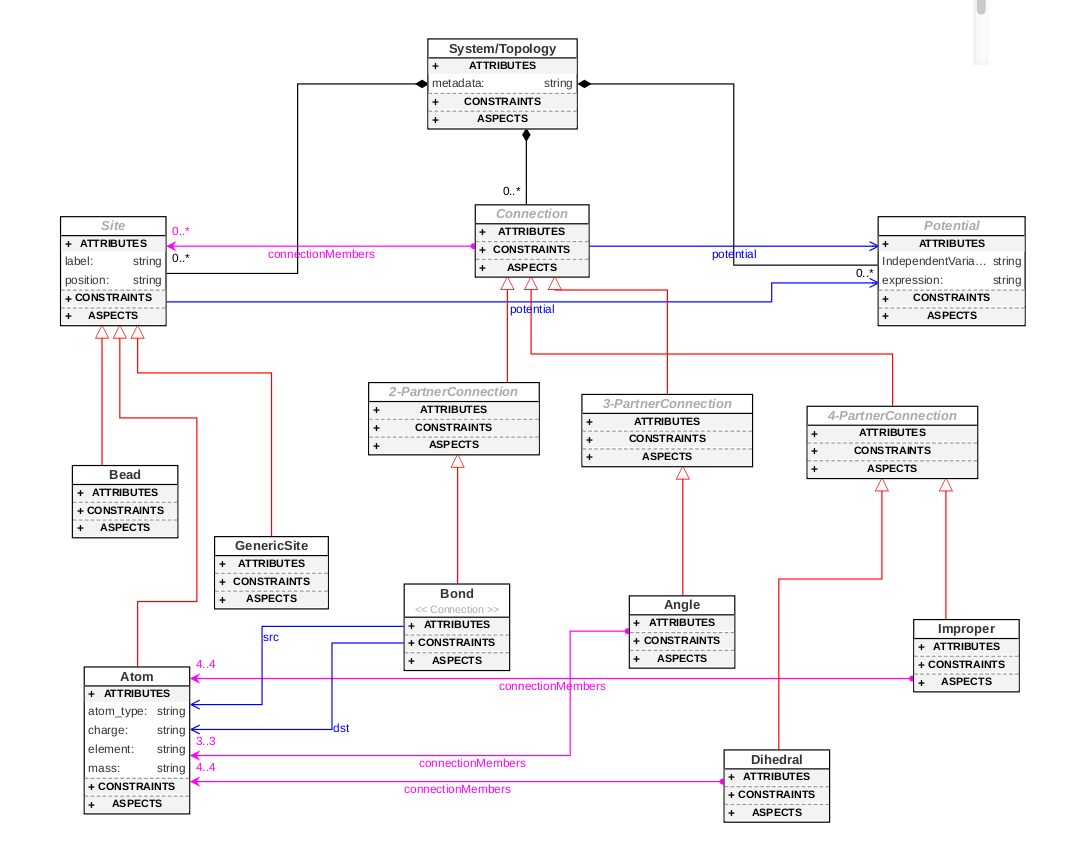
\includegraphics[scale=0.28]{docs/topo}
    \label{fig:TopoDiagram}
\end{figure}
\end{frame}

\begin{frame}[plain]{System Representation Diagrams (II)}

\begin{figure}[]
    \centering
    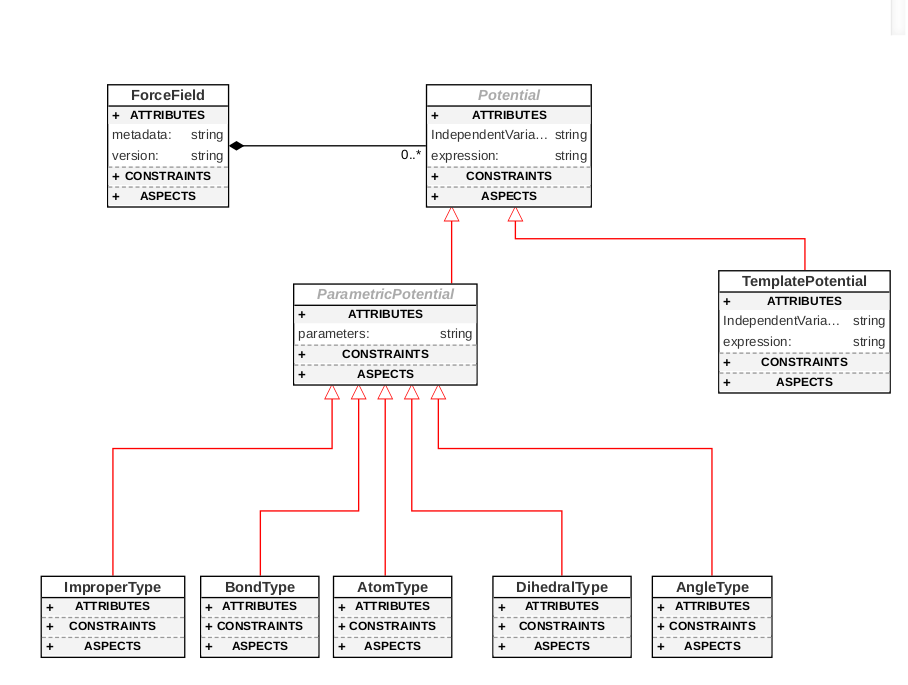
\includegraphics[scale=0.28]{docs/pot}
    \label{fig:TopoDiagram}
\end{figure}
\end{frame}

\section{Next Steps}
\begin{frame}{Next Steps}
    \begin{itemize}
        \item What commonalities exist?
        \item Further define the \texttt{PotentialCollection} file specification
         \item Investigate non-represented systems

    \end{itemize}
\end{frame}

\section{Conclusion}
\begin{frame}{Conclusion}
    \begin{itemize}
        \item \textbf{GPMSO} specification defined above
        \item Extensible base data structures
        \item Data validation for each data structure when applicable
        \item \texttt{PotentialCollection} file format should be human and machine readable
        \item Units required
    \end{itemize}
    \vspace{2em}
    \large \textbf{Any Questions}??
\end{frame}
\end{document}